%&program=xetex
%&encoding=UTF-8 Unicode
%\documentclass[xetex,mathserif,serif]{beamer}
%\documentclass{beamer}
%\documentclass[xetex]{beamer}
\documentclass{beamer}
\usepackage{tikz}
%\setmainfont{Calibri}
% \usepackage{marvosym}
		%\usepackage{fontspec}   %load fonts % xetex
% \usepackage{url,parskip}   %formatting
% \usepackage{xunicode,xltxtra}  %other packages for XeTeX
% \usepackage{titlesec}
% \usepackage{amsmath,amsfonts}
%\font\title="Lohit Tamil:script=taml" at 22pt
% [dvips] allows use of latex->dvips->ps2pdf instead of pdflatex
% [handout] makes something almost appropriate for a hardcopy

%\usepackage{pgfplots}
% packages you might need
%\usepackage{pstricks}
%\usepackage{multido}
%\usepackage{verbatim}
\usepackage{amsmath}
\usepackage{amsfonts}
%\usepackage{psfrag}
%\usepackage{hyperref}


\mode<presentation>
{
  %% these are premade themes
  %% or you can set the inner, outer, color, etc themes below
  %\usetheme{Berkeley}   % left bar
  %\usetheme{Antibes} % tree header
  %\usetheme{Boadilla}  % very plain
  %\usetheme{Warsaw}
  %\usetheme{Copenhagen}
  %\usetheme{Madrid}
  %\usetheme{Rochester} % I like
  %\usetheme{Goettingen}  % right bar
  %\usetheme{Ilmenau}
  \usetikzlibrary{shadows,arrows}
\tikzstyle{materia}=[draw, fill=blue!20, text width=6.0em, text centered,
  minimum height=1.5em,drop shadow]
\tikzstyle{practica} = [materia, text width=18em, minimum width=10em,
  minimum height=3em, rounded corners, drop shadow]

\tikzstyle{materiai}=[draw, fill=green!20, text width=6.0em, text centered,
  minimum height=1.5em,drop shadow]
\tikzstyle{practicai} = [materiai, text width=18em, minimum width=10em,
  minimum height=3em, rounded corners, drop shadow]

\tikzstyle{line} = [draw, thick, color=black!50, -latex']
\newcommand{\practica}[2]{node (p#1) [practica]
  {Step #1\\{\large\textit{#2}}}}

\newcommand{\practicai}[2]{node (p#1) [practicai]
  {Step #1\\{\large\textit{#2}}}}


  %% choose an outertheme: navigation bars etc
  %\useoutertheme{infolines}  % bottom and top bars: HAS SLIDE NUMBERS
  %\useoutertheme{default}
  %\useoutertheme{shadow}
  %\useoutertheme{smoothbars}
  %\useoutertheme{miniframes}
  %\useoutertheme{sidebar}
  \useoutertheme[width=2cm,right]{sidebar}
  %  also [hideallsubsections, hideothersubsections]
  %\useoutertheme{split}  % bottom band and large top outline
  %\useoutertheme{tree}
  %\useoutertheme{smoothtree}

  %% this is an outer theme that Colin wrote that adds page numbers
  %% it seems to work with some of the above themes that don't have a
  %% page number
  \useoutertheme{colinsfoot}  % add bottom bar

  %% the inner theme: bullets styles, etc
  %\useinnertheme{default}  % triangle bullets
  \useinnertheme{rectangles}
  %\useinnertheme{circles}
  %\useinnertheme{rounded}

  %% this will make covered bullets transparent but screws up .eps
  %% (matlab) figures
  %\setbeamercovered{transparent}

  %% color themes: there are lots more, presumably you can make your
  %% own though I've never learned how
  %\usecolortheme{default}
  \usecolortheme{seahorse}
  %\usecolortheme{dolphin}
  %\usecolortheme{albatross}
  %\usecolortheme{beetle}
  %\usecolortheme{dove}
  %\usecolortheme{seagull}
\usepackage{booktabs}

  %% these options effect the style of the "navigation ribbon"
  %\beamertemplatenavigationsymbolsempty
  %\beamertemplatenavigationsymbolsframe
  %\beamertemplatenavigationsymbolsvertical

  %% there are also font theme and various font stuff that I haven't
  %% played with
  %\usefonttheme[onlylarge]{structuresmallcapsserif}
  % \usepackage{times}
  % \usepackage{arev}
}








% some local shortcut math commands
%\renewcommand{\v}[1]{\vec{#1}}
\renewcommand{\v}[1]{\boldsymbol{#1}}
\newcommand{\m}[1]{\text{\textsf#1}}

\newcommand{\dee}{\mathrm{d}}
\newcommand{\dye}{\partial}
\newcommand{\diff}[2]{\frac{\dee #1}{\dee #2}}
\newcommand{\pdiff}[2]{\frac{\dye #1}{\dye #2}}
\newcommand{\grad}{\nabla}
\newcommand{\divergence}{\textsf{div}}
\newcommand{\del}{\nabla}
\newcommand{\delsq}{\nabla^2}
\newcommand{\lap}{\delsq}
%newcommand{\lap}{\Delta}

\newcommand{\dx}{\Delta x}
\newcommand{\dt}{\Delta t}

\newcommand{\scinot}[2]{\ensuremath{#1\times10^{#2}}}

% for pstricks
%\newpsobject{showgrid}{psgrid}{subgriddiv=1,griddots=10,gridlabels=6pt}




\title[Tamil OCR]{OCR for Tamil Language}

\author[\today]{Pradeep Mathesh,CB.EN.U4CSE08131}

\institute[Amrita School of Engineering, External review,Group 52]{%
% Senior undergraduate student,\\
% Department of CSE,\\
% School of Engineering,\\
% Amrita vishwa Vidyapeetham, Coimbatore.
Guide\\
1. Mrs. Hema P Menon, Assistant Professor, CSE\\
2. Dr. K P Soman, Professor, CEN
 }
% \guide[Guide]{%
% 1. Mrs. Hema P Menon, Assistant Professor, CSE
% 2. Dr. K P Soman, Professor, CEN
% }

\date[Talk]{External Review}


%\pgfdeclareimage[height=1.0cm]{university-logo}{sfu-crest}
%\logo{\pgfuseimage{university-logo}}




\begin{document}
    %\setsansfont{Comic Sans MS}
\begin{frame}
  \titlepage
\end{frame}

\frame{
\frametitle{Problem definition}
       \begin{itemize}
		\item To develop a semi-automated Optical character
recognition (OCR) system for Tamil language
			\end{itemize}
}


\begin{frame}
  \frametitle{Tamil OCR}
  "System Architecture"
%       \begin{itemize}
%   \item Page layout analysis
%   \item Noise removal and binarization                          
%   \item Skew correction
%   \item Segmentation
%   \item Classification
%   \item Recognition
%   \item Format reconstruction
%       \end{itemize}

  \begin{figure}\centering
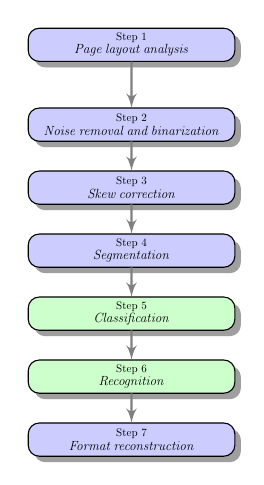
\begin{tikzpicture}[scale=0.4,transform shape]
 
  % Draw diagram elements
  \path \practica {1}{Page layout analysis};
  \path (p1.south)+(0.0,-2) \practica{2}{Noise removal and binarization};
  \path (p1.south)+(0.0,-4) \practica{3}{Skew correction};
  \path (p1.south)+(0.0,-6) \practica{4}{Segmentation};
  \path (p1.south)+(0.0,-8) \practicai{5}{Classification};
  \path (p1.south)+(0.0,-10) \practicai{6}{Recognition};
  \path (p1.south)+(0.0,-12) \practica{7}{Format reconstruction};
    \path [line] (p1.south) -- node [above] {} (p2) ;
    \path [line] (p2.south) -- node [above] {} (p3) ;
    \path [line] (p3.south) -- node [above] {} (p4) ;
    \path [line] (p4.south) -- node [above] {} (p5) ;
    \path [line] (p5.south) -- node [above] {} (p6) ;
    \path [line] (p6.south) -- node [above] {} (p7) ;
%   \path (p3.south)+(5.0,-1.0) \practica{4}{Amplificador para HF};
  \end{tikzpicture}
    \caption{Architecture of a typical OCR system}\label{OCRA}
\end{figure}
\end{frame}


\begin{frame}
  \frametitle{Tamil OCR}
  "Implementations"
      \begin{itemize}
\item Ground truth generating tool - train.py
  \item Blob extraction and preprocessing - createb.py
  \item Recognition engine - hyperplane2.py
  \item Result analyzer - confuse.sh
      \end{itemize}
\end{frame}

\begin{frame}
  \frametitle{Tamil OCR}
  "Input given to tesseract"
\includegraphics[scale=0.6]{./img/input} 
\end{frame}

\frame{
\frametitle{Dataset}
"The dataset is created from two pages of an encyclopedia"
       \begin{itemize}
		\item Training dataset - 4201 blobs
		\item Testing dataset - 4067 blobs
			\end{itemize}
}

\frame{
\frametitle{Ground truth}
"The ground truth is generated using a handy interface"
       \begin{itemize}
		\item Ground truth helps in automating testing
		\item It can used along with "grep" to perform random subsampling.
			\end{itemize}
}

\frame{
\frametitle{Transliteration}
"For easier processing the ground truth is stored in transliterated form."
       \begin{itemize}
		\item 1 a  
		\item 2 A  
		\item 3 i 
		\item 4 I  
		\item ...
			\end{itemize}
}

\frame{
\frametitle{Extraction of blobs}
"Blobs are extracted based on bounding box information given by tesseract"
\begin{table}[!t]\center
\begin{tabular}{cccccc}
\toprule
\textbf{Junk} & \textbf{Top} & \textbf{Left} & \textbf{Right} & \textbf{Bottom} & \textbf{Page no} \\
\midrule
@ &865 & 2893  & 883 & 2913  &0 \\
Q &867 &2875 &878 &2885  &0 \\
w &879 &2875 &889 &2885 &0 \\
w &867 &2852 &881 &2862 &0 \\

\bottomrule
\end{tabular}
  \caption{Sample bounding box information for four blobs in a page}\label{BBOX}
\end{table}
}

\begin{frame}
  \frametitle{Tamil OCR}
  "Sample output after preprocessing"
\includegraphics[scale=0.2]{./img/blobs} 
\end{frame}

\begin{frame}
  \frametitle{Tamil OCR}
  "Ground truth generation"
\includegraphics[scale=0.5]{./img/train} 
\end{frame}


\begin{frame}
  \frametitle{Tamil OCR}
  "Model presented to the recognition engine"
\includegraphics[scale=0.2]{./img/model} 
\end{frame}

\begin{frame}
  \frametitle{Tamil OCR}
  "How model is generated ?"
  \begin{figure}\centering
\includegraphics[scale=0.2]{./img/model_gen} 
  \caption{Model is generated by copying one instance of each of the classes.}
\end{figure}
\end{frame}
\begin{frame}
  \frametitle{Tamil OCR}
  "Feature extraction" \\
  The feature extraction is based on four different
techniques.
        \begin{itemize}
		\item  Active contour model
\item Character geometry
\item Random Projection
\item Hu's Moments
	\end{itemize}
\end{frame}

\frame{
\frametitle{Active contour model}
        \begin{itemize}
		\item Feature is the number of rings
\item Number of points in the contour matrix
\item Maximum length of the contour
	\end{itemize}
}

\frame{
\frametitle{Character geometry}
        \begin{itemize}
		\item Euler Number
\item Regional area
\item Eccentricity
\item Zonal Feature
	\end{itemize}
}

\frame{
\frametitle{Random Projection}
        \begin{itemize}
		\item Common dimensionality reduction technique based
on Random Projection.
\item A form of unsupervised learning. 
\item Object is classified based on L2-norm.
	\end{itemize}
}

\frame{
\frametitle{Hu's Moments}
\begin{itemize}
	\item Decomposing object boundary into line segments

\item The $(p+q)$th order of moment is geometric moment $M_{pq}$ of a gray-level image is defined as


%  \begin{equation}
 $M_{pq} = \int_{-\infty}^\infty\int_{-\infty}^\infty f(x,y)dxdy$\\
%  \end{equation}
\item In the case of a digital image, the double integral of the above equation must be replaced by a summation.

% \begin{equation}
$m_{pq}=\sum_{i=1}^n\sum_{j=1}^ni^pj^qf_{ij}$,\\
% \end{equation}

\item where N is the size of the image and $f_{ij}$ are the grey levels of individual pixels.
\end{itemize}
}

% \frame{
% \frametitle{2D-gabor filter}
%        \begin{itemize}
% 		\item 
% 			\end{itemize}
% }

\frame{
\frametitle{Results}
\begin{table}[!t]\center
  \begin{tabular}{ccc}
\toprule
 \textbf{S.No} & \textbf{Class}  & \textbf{Confusing class}  \\
\midrule
1 &     tu & rru \\  
2 &     vi & li \\  
3 &     va & ya \\  
4 &     wa & ta \\  
5 &     va & na \\  
6 &     va & la \\  
7 &     ku & cu \\  
8 &     mu & zhu \\  
9 &     ku & ru \\  
10 &    pa & pu \\  
11 &    wi & rri \\  
12 &    ki & ci \\  
13 &    ka & ca \\  
\bottomrule
\end{tabular}
  \caption{Samples of least confusing class}\label{LCONF}
  \end{table}
}


\frame{
\frametitle{Results}
\begin{table}[!t]\center
  \begin{tabular}{ccc}
\toprule
\textbf{Class}  & \textbf{Minimum} & \textbf{Maximum} \\
\midrule
ku & 263 & 294 \\  
ru & 258 & 280 \\  
tu & 256 & 282 \\  
rru & 243 & 262 \\  
vi & 227 & 288 \\  
li & 244 & 259 \\  
ya & 186 & 210 \\  
na & 239 & 287 \\  
ta & 246 & 256 \\  
va & 245 & 264 \\  
wa & 212 & 231 \\  
ka & 212 & 225 \\  
ca & 146 & 200 \\  
\bottomrule
\end{tabular}
  \caption{Min and max no. of contour points for the least confusing classes}\label{MMAX}
\end{table}

}



% \frame{
% \frametitle{}
%        \begin{itemize}
% 		\item 
% 			\end{itemize}
% }
\begin{frame}
  \frametitle{Tamil OCR}
  "Work done"
          \begin{itemize}
  \item A Ground truth generating tool has been written
  \item A recognition engine has been implemented based on i) random projection technique (RPT) and ii) SVM training and classification.
  \item A result analysing script for RPT has been implemented
          \end{itemize}
\end{frame}


\begin{frame}
  \frametitle{Tamil OCR}
  "Work done"
        \begin{itemize}
	\item Comparison of SVMTC and RPT is done
  \item Inspection of confusing classes for hierarchal classification to improve the accuracy
  \item The least confusing classes were picked

  \item Possible cases are
%       \setsansfont{Lohit Tamil:script=taml}
%   (க->ச 111),(ச->க 5),(இ->பி 8),(ரு->கு 9)
%     \setsansfont{Comic Sans MS}
  \includegraphics[scale=0.4]{./img/conf} 
  \item Currently, the classification is done solely based on level set method.
  \item The features that are used to discriminate confusing classes are number of rings and points of the contour matrix.
        \end{itemize}
\end{frame}



\begin{frame}
  \frametitle{Tamil OCR}
  "Some elusive samples"
\begin{center}
\begin{tabular}{ | c | c |}
\hline
\includegraphics[scale=0.1]{./img/ya} &

\includegraphics[scale=0.1]{./img/nu} \\ \hline
\includegraphics[scale=0.1]{./img/tu} &
\includegraphics[scale=0.1]{./img/la} \\
\hline
\end{tabular}
\end{center}
\end{frame}

\begin{frame}
  \frametitle{Tamil OCR}
  "Result"
\begin{center}
\begin{tabular}{ | l | l | l | l | l | l |}
\hline
& &  \multicolumn{2}{|c|}{Samples}&\multicolumn{2}{|c|}{Accuracy} \\ \hline
S.No & Features &  Training &Testing & Training & Testing \\ \hline
1* & 555 & 4201 & 4067 & 75 & $<$ 44 (3 classes) \\ \hline
2** & 1000 & 155 classes& 4201 & 98 & 59 \\
\hline
\end{tabular}

\end{center}
        \begin{itemize}
	  \item Legend
  \item *Structural and Statistical features (SVM trainer and classifier is used for classification)
\item **Random Projection (L2-norm is used for recognition)
      \end{itemize}
\end{frame}


\begin{frame}
  \frametitle{Tamil OCR}
  "False positives and negatives"
  
%   \subsection{Confusion matrix}
\begin{figure}\centering
\includegraphics[scale=0.4]{./img/confuse}
  \caption{Sample confusion matrix}\label{CONF}
\end{figure}


%         \begin{itemize}
% 	      \setsansfont{Lohit Tamil:script=taml}
% 	\item 
	
% 	 அ:
% அ->அ 40
% ஆ->அ 1
%  ஆ:
% அ->ஆ 1
% ஆ->ஆ 33
%  இ:
% இ->இ 41
%  ஈ:
% ஈ->ஈ 1
% ா->ஈ 1
%  உ:
% உ->உ 24
% ப->உ 1
% ல->உ 4
% வ->உ 4
%  ஊ:
  %\item Integrating level set method with random projection technique for hierarchal classification.
%         \end{itemize}
	
\end{frame}

\frame{
\frametitle{Future enhancement}
"Improving the accuracy"
       \begin{itemize}
		\item Rigorous analysis of hierarchal classification can be carried out to improve the accuracy.
			\end{itemize}
}

    %\setsansfont{Comic Sans MS}

\begin{frame}
  \frametitle{Tamil OCR}
  "Reference"
\begin{thebibliography}{10}
  \bibitem{IEEEhowto:lauer}
F. Lauer ,”MSVMpack: a Multi-Class Support Vector Machine Package”, http://www.loria.fr/~lauer/MSVMpack,2011
  \bibitem{IEEEhowto:kaihua}
   Kaihua Zhang.et.al,"Active contours with selective local or global segmentation: a new variational approach and
   level set method",Image and Vision Computing, 2010. 
  \bibitem{IEEEhowto:bresson}
  Xavier Bresson, “A Short Guide on a Fast Global Minimization Algorithm for Active Contour Models”, April 22, 2009
\end{thebibliography}
\end{frame}


\begin{frame}
  \frametitle{Tamil OCR}
\begin{thebibliography}{10}

\bibitem{IEEEhowto:shi}
Qinfeng Shi, “Rapid Face Recognition Using Hashing”, Australian National University, and NICTA
      Canberra, Australia, 2009
\bibitem{IEEEhowto:dileep}
Dinesh Dileep, "A feature extraction technique based on character geometry for character recognition", http://www.ece.iisc.ernet.in/~dileep, 2008

\bibitem{IEEEhowto:pradeep}
Ray Smith, "An Overview of the Tesseract OCR Engine", IEEE Trans., 2007


\bibitem{IEEEhowto:flusser}
Jan Flusser and Tomas Suk, “On the Calculation of Image Moments”, Institute of Information Theory and Automation, Academy of Sciences of the Czech Republic, January,1999
\end{thebibliography}
\end{frame}

\begin{frame}
  \frametitle{Tamil OCR}
\begin{thebibliography}{10}

\bibitem{krish}
V. Krishnamoorthy, "OCR Software for Printed Tamil Text", 
Proceedings of Tamil Internet 2002, California, USA, 2002

\bibitem{anbu}
Anbumani Subramanian and Bhadri Kubendran,"Optical Character Recognition of Printed Tamil Characters",
http://www.ece.vt.edu/,2000
\bibitem{flusser2}
Jan Flusser et.al,"Moments and Moment Invariants in Pattern Recognition",ISBN 978-0-470-69987-4,Page.no 49,2009

\end{thebibliography}
\end{frame}


% \begin{frame}
%   \frametitle{Bullet points}
%   \framesubtitle{\ldots using \LaTeX}

%   \begin{itemize}
%     \item Colin rocks at \LaTeX
%     \item this isn't boring:
%       \begin{align*}
%         \phi_t = -w \cdot \grad \phi
%       \end{align*}
%   \end{itemize}

% \end{frame}




% \begin{frame}
%   \frametitle{Bibliography}
% \begin{thebibliography}{10}
% \bibitem{beamerUserGuide}[Beamer User Guide]
%   Till Tantau
%   \newblock \emph{User's Guide to the Beamer Class}.
% \end{thebibliography}
% \end{frame}


\frame{
\frametitle{Questions ?}
\begin{center}
%        \begin{itemize}
\includegraphics[scale=0.5]{./img/comp}
% 			\end{itemize}
\end{center}
}
\end{document}
